\section*{Chapitre 8}
\section{Ce que nous ...}
\indent Dans ce chapitre, nous aborderons dans une première partie sur un point que nous n'avons pas eu le temps de développer :  la fonctionnalité d’apprentissage au chatbot. Dans deuxième partie, nous détaillerons les aspects du projet qu'il reste à développer pour faire de notre travail une réelle application commercialisable.

\subsection{... Aurions du faire}
\indent Nous verrons dans cette partie une fonctionnalité que nous n'avons pas eu le temps de réaliser : la fonctionnalité d'apprentisage au chatbot.

\subsubsection{Apprentissage au chatbot}
\indent Avant de commencer notre PAO, nous avons proposé une fonctionnalité dans notre liste de fonctionnalités à réaliser : Apprentissage au chatbot. Traduit en français courant, nous voulons que notre chatbot puisse apprendre au cours d'écouter et répondre à l'utilisateur. 

\begin{lstlisting}[frame=none,aboveskip=0.5em]
<aiml version="1.0.1" encoding="UTF-8">
   <category>
      <pattern>MY DOGS NAME IS *</pattern>
      <template>
         That is interesting that you have a dog named <set name="dog"><star/></set>
      </template>  
   </category>  
   <category>
      <pattern>WHAT IS MY DOGS NAME</pattern>
      <template>
         Your dog's name is <get name="dog"/>.
      </template>  
   </category>  
</aiml>
\end{lstlisting}

\indent C'est un exemple pour vous montrer notre idée principale. Avec cette fonctionnalité, notre chatbot peut aquérir les informations de l'extérieur.

\indent Nous avons fait un diagramme de séquence aussi pour expliquer notre idée. Malheureusement, à cause de la manque de temps et de technique, nous avons pas réalisé cette fonctionnalité, nous espérons que le groupe suivant peut la faire. 

\begin{figure}[h]
\centering
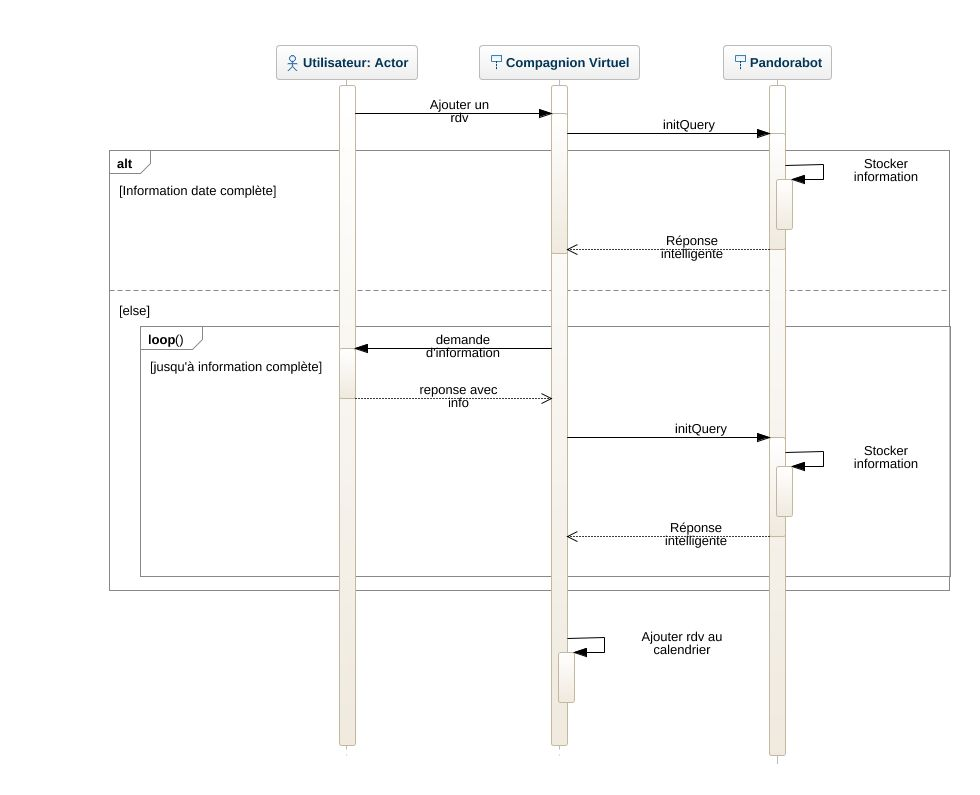
\includegraphics[width=1\linewidth]{./diagrammes/SequenceDiagram_multi_conversation.jpeg}
\caption{Diagramme de sequence d'apprentissage au chatbot.\label{fig4}}
\end{figure}
\newpage

\subsection{... pourrions faire par la suite}
\indent Dans cette partie, nous vous proposerons des problématiques de travail à effectuer pour faire en sorte que notre application soit la plus complète possible. Les points qui seront détaillés ne forment pas une liste exhaustive de ce qui pourrait être fait sur l'application mais constitue une base de réflexion sur ce qui paraît être important de développer ou d'améliorer, afin de permettre à une autre équipe de reprendre le projet afin de le terminer.

\subsubsection{Améliorer l'interface d'utilisateur encore}
\indent Vue que nous avons déjà travaillé sur ce problématique, nous pensons que l'interface d'utilisateur de notre application a été amélioré. Cependant, étant comparée avec les applications comerciales de compagnon virtuel, par exemple : siri, cortana, notre interface d'utilisateur n'est pas assez belle et moderne. Nous souhaitons que la prochaine équipe peut travailler au dessus.

\subsubsection{Ajout des fonctionnalités quotidiennes}
\indent Au début du semestre, personnellement, nous pensions à ajouter la fenêtre des nouvelles et la prévision météorologique dans l'interface de notre application car ces fonctionnalités appraitent dans les autres compagnons virtuels comerciales. Avec ces fonctionnalités, notre application va donner une meilleure expérience d'utilisateur.

\subsubsection{Gestion de la langue du compagnon virtuel}
\indent Enfin une fonctionnalité supplémentaire pourrait être de permettre à l'utilisateur de choisir une langue par défaut puis de la modifier par la suite. L'ajout de la gestion de la langue du compagnon virtuel peut être une fonctionnalité supplémentaire intéressante si nous voulons que les gens avec différentes nationalités utlisent notre application.
